\quad \quad In this chapter we will deal with the three kinds of multiplication with vectors. By far the easiest would be scaling a vector. As we have previously discussed, the magnitude of a vector is the length of a vector. But what if I want to "elongate" the vector by some amount to make it longer or shorter. This is called \textit{scaling}.
\begin{figure}[h]
 \centering
 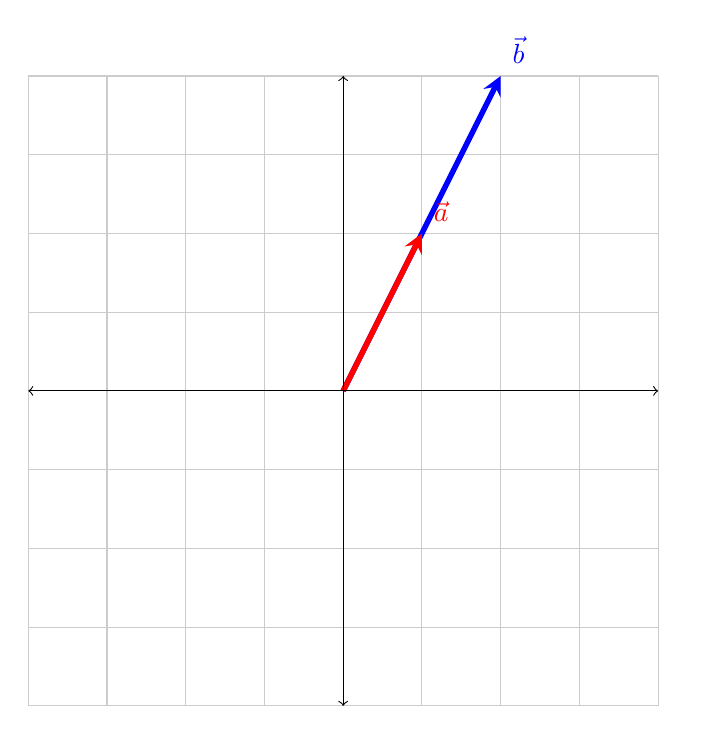
\begin{tikzpicture}
    \draw[thin, gray!40] (-4,-4) grid (4,4);
    \draw[line width=2pt, blue, -stealth] (0,0) -- (2,4) node[anchor=south west]{\(\vec{b}\)};
    \draw[line width=2pt, red, -stealth] (0,0) -- (1,2) node[anchor=south west]{\(\vec{a}\)};
    \draw[<->] (-4,0) -- (4,0) node[right]{\(\ihat\)};
    \draw[<->] (0,-4) -- (0,4) node[above]{\(\jhat\)}; 
 \end{tikzpicture}
 \caption{Two vectors, one twice as long as the other.}

 \label{scalevector}
\end{figure}


Take a look at \Cref{scalevector}, \(\vec{b}\) is twice as long as \(\vec{a}\). What should we multiply to \(\vec{a}\) to make as long as \(\vec{b}\)? If you guessed 2, the you are right. To multiply a vector by a constant, we multiply each individual component of the vector by the constant. From the figure, we can identify that \(\vec{a}=\begin{bsmallmatrix}
  1 \\
  2
\end{bsmallmatrix}\) so \(2\vec{a} = \begin{bsmallmatrix}
  2 \times 1 \\
  2 \times 2
\end{bsmallmatrix} = \begin{bsmallmatrix}
  2 \\
  4
\end{bsmallmatrix}\) which is equal to \(\vec{b}\). You may extrapolate this to higher dimensions.
\begin{definition}
  Scaling a n-dimensional vector \(\vec{v}\) by a constant \(n\) is defined as such:
  \begin{equation*}
    n\vec{v} = n \begin{bsmallmatrix}
      v_1 \\
      \dots \\
      v_n
    \end{bsmallmatrix} = \begin{bsmallmatrix}
      n \times v_1 \\
      \dots \\
      n \times v_n
    \end{bsmallmatrix}
  \end{equation*}
\end{definition}
Let us try something fun, what if we multiplied the vector by a negative number? Well, the computation remains the same.
\begin{marginfigure}
  \centering
  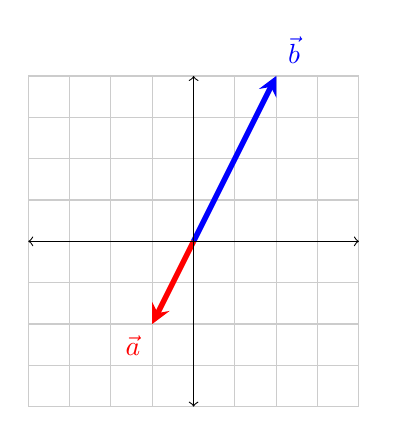
\begin{tikzpicture}[scale=0.525]
    \draw[thin, gray!40] (-4,-4) grid (4,4);
    \draw[line width=2pt, blue, -stealth] (0,0) -- (2,4) node[anchor=south west]{\(\vec{b}\)};
    \draw[line width=2pt, red, -stealth] (0,0) -- (-1,-2) node[anchor=north east]{\(\vec{a}\)};
    \draw[<->] (-4,0) -- (4,0) node[right]{\(\ihat\)};
    \draw[<->] (0,-4) -- (0,4) node[above]{\(\jhat\)}; 
 \end{tikzpicture}
 \caption{Two vectors, one is scaled by -0.5.}

 \label{scalevectorneg}
\end{marginfigure} 
As you can see from \Cref{scalevectorneg}, \(\vec{a}=(-0.5)\vec{b}\). You may wish to compute this yourself to verify. One thing to note here is that the vector gets flipped across the origin when the constant the vector is multiplied to is negative. Also, when scaling a vector by some constant, the reader may want to verify using \Cref{vecmagnitude} that the magnitude of the vector is also scaled by that constant. This should be a trivial proof.


You may have noticed that I have abstained from using either the \(\cdot \) or \(\times \) operators. The reason is bad notation which is sprinkled throughout mathematics. These two operators have special meanings in the realm of linear algebra. We shall first explore the easier one, the \textit{dot product}.
\newpage


Dot products use the \(\cdot\) operator and only acts on vectors, do not abuse notation by using the \(\cdot\) operator in the context of scaling a vector. Dot products are actually fairly straightforward to compute:

\begin{definition}
  The dot product of two vectors in n-dimensional space \(\vec{a}\) and \(\vec{b}\) is:
  \begin{equation*}
    \vec{a} \cdot \vec{b} = a_1 b_1 + a_2 b_2 + \dots + a_n b_n = (||\vec{a}||)(||\vec{b}||)\cos{\theta} 
  \end{equation*}
  where \(\theta\) is the angle between the two vectors.
  \label{dotproduct}
\end{definition}

From \Cref{dotproduct}, we can tell that the dot product tells us something about the relationship between the two vectors. 

\begin{figure}[h]
  \centering
  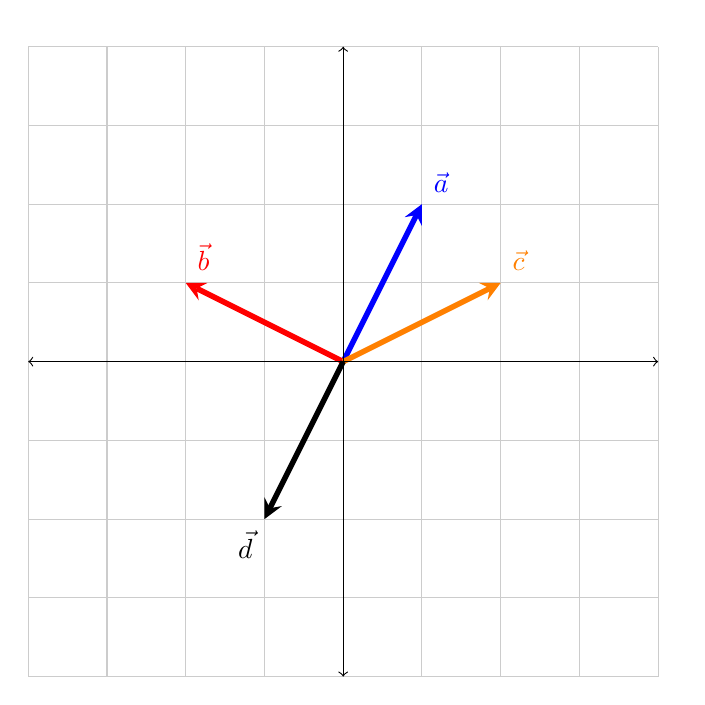
\begin{tikzpicture}
    \draw[thin, gray!40] (-4,-4) grid (4,4);
    \draw[line width=2pt, blue, -stealth] (0,0) -- (1,2) node[anchor=south west]{\(\vec{a}\)};
    \draw[line width=2pt, red, -stealth] (0,0) -- (-2,1) node[anchor=south west]{\(\vec{b}\)};
    \draw[line width=2pt, orange, -stealth] (0,0) -- (2,1) node[anchor=south west]{\(\vec{c}\)};
    \draw[line width=2pt, black, -stealth] (0,0) -- (-1,-2) node[anchor=north east]{\(\vec{d}\)};
    \draw[<->] (-4,0) -- (4,0) node[right]{\(\ihat\)};
    \draw[<->] (0,-4) -- (0,4) node[above]{\(\jhat\)}; 
  \end{tikzpicture}
  \caption{Four vectors pointing in different directions.}
  \label{dotproductfig}
\end{figure}

Firstly, note down the components of each vector in \Cref{dotproductfig}. Then, let us compute \(\vec{a}\cdot \vec{b}\). By \Cref{dotproduct}, it is \(1(-2)+2(1)=0\). Also, it is important to take note that these two vectors are orthogonal(at right angles with each other). This brings us to an important property of dot products, if two vectors are orthogonal, then their dot product is 0. This can be seen from the fact that \(\cos(\frac{\pi}{2})=0\) and from the second definition of dot products in \Cref{dotproduct}. In a sense, the dot product tells you how aligned are the directions of two vectors. Another example would be taking the dot product of two identical vectors, such as \(\vec{a}\cdot\vec{a}\). The dot product there is \(1(1)+2(2)=5\). In addition, we know \(\cos{0}=1\) so according to the second definition, \(\vec{a}\cdot\vec{a}=(||\vec{a}||)(||\vec{a}||)=(||\vec{a}||)^{2}\). If we take the square root on both sides, \(||\vec{a}||=\sqrt{\vec{a}\cdot\vec{a}}\) which can be rewritten as \(||\vec{a}||=\sqrt{a_{1}^{2}+\dots+a_{n}^{n}}\). This is exactly the formula we got in \Cref{vecmagnitude} for the magnitude of a vector. This is a pretty nice result.
\begin{example}
  From \ref{dotproductfig}, we can see that:
  \begin{equation*}
    \vec{a} \cdot \vec{c} = \begin{bmatrix}
      1 \\
      2
    \end{bmatrix} \cdot \begin{bmatrix}
      2 \\
      1
    \end{bmatrix} = 1(2) + 2(1) = 4
  \end{equation*}
  \begin{equation*}
    \vec{a} \cdot \vec{d} = \begin{bmatrix}
     1 \\
     2
    \end{bmatrix} \cdot \begin{bmatrix}
      -1 \\
      -2
    \end{bmatrix} = 1(-1) + 2(-2) = -5
  \end{equation*}
\end{example}
\begin{remark}
  Generally, when finding the dot product, we use the first form in \ref{dotproduct} as it is typically easier to compute. It is also important to know that the dot product of two vectors results in a number, not a vector like in scaling.
\end{remark}


Next, we will move on to the more difficult concept: \textit{Cross product}. This is a uniquely three dimensional topic. In a nutshell, the cross product of two products results in a vector that is both perpendicular to the two vectors and has the magnitude of the area of a parallelogram whose sides are the two vectors

